\documentclass[11pt]{article}
\usepackage[T1]{fontenc}
\usepackage{lmodern}
\usepackage[margin=1in]{geometry}
\usepackage{amsmath,amssymb,booktabs,longtable,graphicx,url,fancyvrb,float,etoolbox}
\setlength{\LTpre}{8pt}\setlength{\LTpost}{8pt}
% Backport the finite-shrink fix in LaTeX tools longtable v4.25 (issue 1907).
% No-op when the installed version already uses finite shrink.
\makeatletter
\patchcmd{\LT@output}{\vss}{\vskip\z@\@plus1fil\@minus\normalbaselineskip}{}{}
\patchcmd{\LT@output}{\vss}{\vskip\z@\@plus1fil\@minus\normalbaselineskip}{}{}
\makeatother
\usepackage[protrusion=true,expansion=false]{microtype}
\title{RL-BCM: Detailed Experiments and Reproducibility Report}
\author{Hieu B. Pham, Uyen T. Nguyen, Canh V. Pham\\[2pt]\small Companion report to ``Reinforcement Learning for Betweenness Centrality\\\small Maximization via Graph Structure Modification'' (CSoNet 2026)}
\date{September 2026}
\begin{document}\maketitle
This report contains additional measured results and implementation details
for the CSoNet 2026 paper. The paper is self-contained for its principal
claims. All reported experiments were executed locally; unrun baselines are
explicitly marked as such.
\tableofcontents

\section{Scope}
Full Greedy is stronger
than RL in all three synthetic-family means, and the learned myopic control is
also stronger than the long-horizon model. The results support a learned
heuristic with a measurable quality/cost profile, not a demonstrated planning
advantage. All methods use the same relative-gain definition, with the
initial BC as denominator.

The protocol uses held-out validation, deterministic SHA-256 dataset
seeds, dropout-free PPO likelihoods, a remaining-budget feature,
unordered symmetric edge scores, and absolute terminal-aligned reward.
The exact task adds a fixed number of edges; at-most-budget behavior is audited
separately because BC is not monotone under unrestricted insertion.

\section{Frozen experimental design}
Training uses 480 graphs, validation 36, and test 240. Synthetic configurations
are ER with probabilities 0.1/0.2, BA with attachment 2/3, and WS with
degree--rewiring pairs (4,0.1)/(6,0.2). Connectedness rejection is explicit.
Train sizes are 20,30,40,50; test sizes are 30,50,80,100. Each test family has
two configurations, four sizes, and ten graphs per cell. Targets come from the
bottom quartile of positive BC. Saved graph hashes verify disjoint splits.

Five seeds (11,22,33,44,55) are trained for each of exact-BC, no-BC-input,
and gamma-zero models. Every run executes 5,000 episodes of five decisions.
All variants use three width-64 mean GraphSAGE layers, a 192--64--32--1 edge
MLP, a 128--64--1 value head, and the same optimizer settings. Adam uses
$3\cdot10^{-4}$; PPO uses clip 0.2, four epochs, minibatches of 32, 16 episodes
per rollout, entropy 0.01, value coefficient 0.5, gradient clipping 0.5, and
GAE lambda 0.95. Main gamma is one; the control changes only gamma to zero.
The final checkpoint is used without test or validation selection.

\section{Metric definitions and uncertainty}
Primary outcomes are normalized endpoint-excluding final BC and its absolute
increase. Relative increase is $(B_k-B_0)/B_0$ only for $B_0>10^{-12}$.
The mean of relative increases is not a ratio of means and can be dominated
by small initial values. We report median relative gain as a secondary metric.

For learned models the measurement matrix has five seed rows and graph columns.
The crossed bootstrap independently samples seed indices and graph indices,
using the same sampled graph columns for both members of a contrast. Graphs
are stratified by configuration and size. We use 10,000 replicates with fixed
bootstrap seed 92831. This estimates both observed training-run and test-graph
variation; it does not incorporate new training corpora or new network families.
For deterministic baselines, only graph columns vary. Original Random and global-sampled
baselines have one predefined randomization per graph, so their within-graph
randomization variance is not independently estimated.

Seed-level sign-flip tests use graph-averaged paired differences and all 32
sign assignments. They are two-sided, require a symmetric null for these
differences, and have minimum attainable unadjusted $p=0.0625$. Holm correction
is applied across ER, BA, and WS for each specified comparator. A bootstrap
interval excluding zero and a coarse sign-flip p-value need not agree: the
two procedures use different sampling assumptions and resolution. We do not
describe this discrepancy as proof of statistical significance.

\section{Full primary and secondary metrics}
\begin{longtable}{llrrrr}
\toprule Family & Method & $B_0$ & $B_k$ & $B_k-B_0$ & Median rel. (\%)\\ \midrule\endhead
ER & RL-BCM & 0.00747 & 0.08007 & 0.07260 & 620.8\\
ER & RL without BC & 0.00747 & 0.07848 & 0.07101 & 622.1\\
ER & RL myopic & 0.00747 & 0.08086 & 0.07339 & 648.2\\
ER & Full Greedy & 0.00747 & 0.08355 & 0.07608 & 640.0\\
ER & Incident Greedy & 0.00747 & 0.08355 & 0.07608 & 640.0\\
ER & Sampled Greedy (20) & 0.00747 & 0.04004 & 0.03257 & 164.1\\
ER & Sampled Greedy (100) & 0.00747 & 0.07022 & 0.06275 & 398.0\\
ER & Degree & 0.00747 & 0.04560 & 0.03814 & 244.6\\
ER & Random & 0.00747 & 0.00889 & 0.00142 & -1.4\\
BA & RL-BCM & 0.00203 & 0.06278 & 0.06075 & 3085.6\\
BA & RL without BC & 0.00203 & 0.06412 & 0.06209 & 3162.2\\
BA & RL myopic & 0.00203 & 0.06630 & 0.06427 & 3260.9\\
BA & Full Greedy & 0.00203 & 0.07134 & 0.06930 & 3526.4\\
BA & Incident Greedy & 0.00203 & 0.07134 & 0.06930 & 3526.4\\
BA & Sampled Greedy (20) & 0.00203 & 0.02225 & 0.02022 & 759.9\\
BA & Sampled Greedy (100) & 0.00203 & 0.05144 & 0.04940 & 2610.9\\
BA & Degree & 0.00203 & 0.02369 & 0.02165 & 940.9\\
BA & Random & 0.00203 & 0.00310 & 0.00107 & -1.1\\
WS & RL-BCM & 0.01263 & 0.26387 & 0.25124 & 1927.6\\
WS & RL without BC & 0.01263 & 0.25919 & 0.24656 & 1953.8\\
WS & RL myopic & 0.01263 & 0.26778 & 0.25515 & 1994.5\\
WS & Full Greedy & 0.01263 & 0.28227 & 0.26964 & 2119.9\\
WS & Incident Greedy & 0.01263 & 0.28227 & 0.26964 & 2119.9\\
WS & Sampled Greedy (20) & 0.01263 & 0.12735 & 0.11472 & 733.5\\
WS & Sampled Greedy (100) & 0.01263 & 0.23348 & 0.22085 & 1674.0\\
WS & Degree & 0.01263 & 0.20811 & 0.19548 & 1534.7\\
WS & Random & 0.01263 & 0.01654 & 0.00391 & -4.2\\
\bottomrule\end{longtable}
\subsection{All training-seed means}
\begin{table}[H]
\centering
\caption{Mean final BC per training seed on the same 80 graphs per family. SD is between the five seed means, not between graph instances.}
\label{tab:seeds}
\small
\setlength{\tabcolsep}{3pt}
\begin{tabular}{lrrrrrr}
\toprule
Family / model & 11 & 22 & 33 & 44 & 55 & SD \\
\midrule
ER / RL-BCM & 0.0809 & 0.0803 & 0.0796 & 0.0793 & 0.0802 & 0.0006 \\
ER / RL without BC & 0.0790 & 0.0782 & 0.0784 & 0.0788 & 0.0780 & 0.0004 \\
ER / RL myopic & 0.0810 & 0.0808 & 0.0818 & 0.0794 & 0.0812 & 0.0009 \\
BA / RL-BCM & 0.0612 & 0.0641 & 0.0630 & 0.0622 & 0.0634 & 0.0011 \\
BA / RL without BC & 0.0620 & 0.0658 & 0.0632 & 0.0634 & 0.0663 & 0.0018 \\
BA / RL myopic & 0.0667 & 0.0661 & 0.0649 & 0.0671 & 0.0667 & 0.0009 \\
WS / RL-BCM & 0.2671 & 0.2691 & 0.2639 & 0.2581 & 0.2611 & 0.0044 \\
WS / RL without BC & 0.2498 & 0.2528 & 0.2702 & 0.2600 & 0.2631 & 0.0082 \\
WS / RL myopic & 0.2693 & 0.2574 & 0.2698 & 0.2727 & 0.2697 & 0.0060 \\
\bottomrule
\end{tabular}
\end{table}

\begin{figure}[H]\centering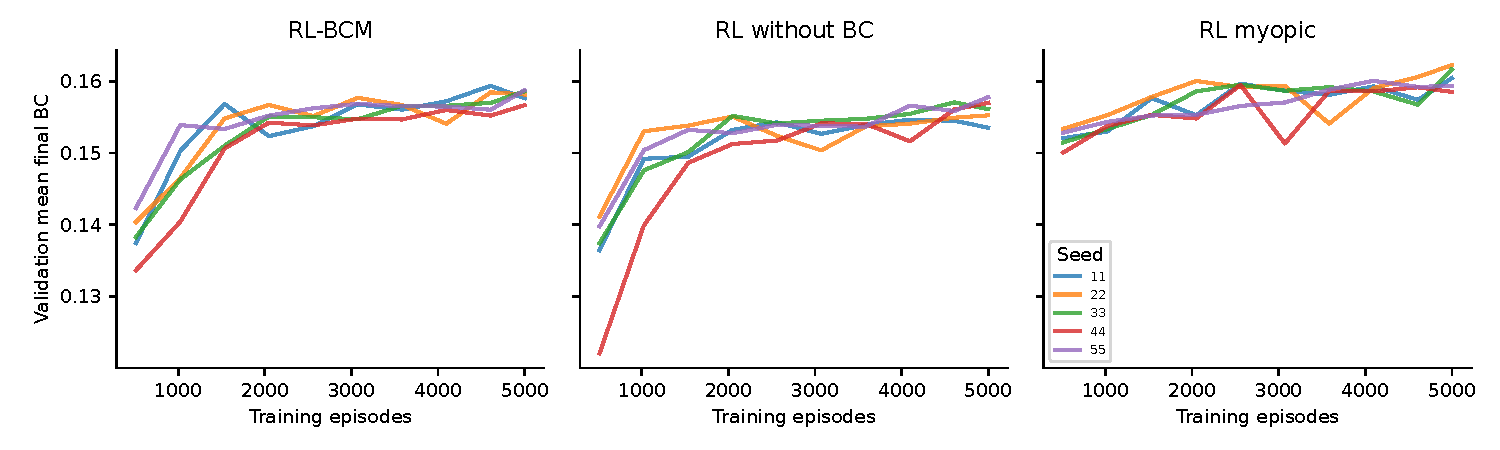
\includegraphics[width=\textwidth]{figures/training.pdf}\caption{Held-out validation for all seeds; final checkpoints are used without selection.}\end{figure}
\subsection{Paired comparisons}
\begin{longtable}{llrrrrr}
\toprule Family & Contrast & Difference & 95\% CI & Win\% & Tie\% & $p_H$\\ \midrule\endhead
ER & exact - FullGreedy & -0.00348 & [-0.00479,-0.00228] & 6.5 & 6.2 & 0.188\\
ER & exact - IncidentGreedy & -0.00348 & [-0.00479,-0.00228] & 6.5 & 6.2 & 0.188\\
ER & exact - Degree & +0.03446 & [+0.02988,+0.03951] & 100.0 & 0.0 & 0.188\\
ER & exact - no\_bc & +0.00159 & [+0.00064,+0.00267] & 63.7 & 10.5 & 0.188\\
ER & exact - myopic & -0.00079 & [-0.00184,+0.00015] & 34.0 & 11.5 & 0.188\\
BA & exact - FullGreedy & -0.00856 & [-0.00990,-0.00726] & 2.5 & 2.8 & 0.188\\
BA & exact - IncidentGreedy & -0.00856 & [-0.00990,-0.00726] & 2.5 & 2.8 & 0.188\\
BA & exact - Degree & +0.03909 & [+0.03643,+0.04189] & 99.8 & 0.0 & 0.188\\
BA & exact - no\_bc & -0.00134 & [-0.00246,-0.00022] & 35.2 & 12.2 & 0.188\\
BA & exact - myopic & -0.00352 & [-0.00511,-0.00196] & 20.2 & 11.8 & 0.188\\
WS & exact - FullGreedy & -0.01840 & [-0.02243,-0.01446] & 11.5 & 0.0 & 0.188\\
WS & exact - IncidentGreedy & -0.01840 & [-0.02243,-0.01446] & 11.5 & 0.0 & 0.188\\
WS & exact - Degree & +0.05576 & [+0.04573,+0.06609] & 95.5 & 0.0 & 0.188\\
WS & exact - no\_bc & +0.00468 & [-0.00409,+0.01399] & 46.5 & 3.2 & 0.500\\
WS & exact - myopic & -0.00391 & [-0.01116,+0.00488] & 32.5 & 2.8 & 0.438\\
\bottomrule\end{longtable}
\subsection{Breakdown by graph size}
\begin{longtable}{lrrrrrrr}
\toprule Family, $n$ & Degree & SG20 & SG100 & Full G. & RL & No BC & Myopic\\ \midrule\endhead
ER, 30 & 0.12742 & 0.11566 & 0.19457 & 0.21863 & 0.21020 & 0.20753 & 0.21191\\
ER, 50 & 0.03295 & 0.02755 & 0.05720 & 0.07053 & 0.06705 & 0.06508 & 0.06802\\
ER, 80 & 0.01331 & 0.01078 & 0.01813 & 0.02803 & 0.02677 & 0.02576 & 0.02706\\
ER, 100 & 0.00874 & 0.00615 & 0.01097 & 0.01699 & 0.01625 & 0.01554 & 0.01644\\
BA, 30 & 0.03592 & 0.05003 & 0.09769 & 0.10641 & 0.10211 & 0.09968 & 0.10316\\
BA, 50 & 0.02333 & 0.02472 & 0.05566 & 0.07624 & 0.07032 & 0.07041 & 0.07280\\
BA, 80 & 0.01870 & 0.00833 & 0.03003 & 0.05498 & 0.04324 & 0.04663 & 0.04822\\
BA, 100 & 0.01681 & 0.00592 & 0.02236 & 0.04771 & 0.03545 & 0.03976 & 0.04103\\
WS, 30 & 0.22493 & 0.17998 & 0.27979 & 0.28766 & 0.28142 & 0.28010 & 0.28217\\
WS, 50 & 0.21272 & 0.14489 & 0.25138 & 0.28792 & 0.27873 & 0.27588 & 0.28282\\
WS, 80 & 0.21265 & 0.11507 & 0.22262 & 0.28504 & 0.26407 & 0.25930 & 0.27049\\
WS, 100 & 0.18214 & 0.06944 & 0.18013 & 0.26845 & 0.23126 & 0.22147 & 0.23564\\
\bottomrule\end{longtable}
\subsection{At-most-budget diagnostic}
The following means select the best prefix of the stored five-step trajectory, including no modification. This is an oracle-assisted diagnostic, not a separately trained stopping policy. No-BC deployment would require additional BC evaluation to choose such a prefix.
\begin{longtable}{llrr}
\toprule Family & Method & Fixed budget & Best prefix\\ \midrule\endhead
ER & Degree & 0.045605 & 0.045605\\
ER & Full Greedy & 0.083545 & 0.083545\\
ER & RL-BCM & 0.080069 & 0.080069\\
ER & RL without BC & 0.078477 & 0.078477\\
ER & RL myopic & 0.080857 & 0.080857\\
BA & Degree & 0.023688 & 0.023688\\
BA & Full Greedy & 0.071335 & 0.071335\\
BA & RL-BCM & 0.062780 & 0.062780\\
BA & RL without BC & 0.064123 & 0.064123\\
BA & RL myopic & 0.066304 & 0.066304\\
WS & Degree & 0.208111 & 0.208111\\
WS & Full Greedy & 0.282269 & 0.282269\\
WS & RL-BCM & 0.263868 & 0.263868\\
WS & RL without BC & 0.259187 & 0.259187\\
WS & RL myopic & 0.267780 & 0.267780\\
\bottomrule\end{longtable}
\section{Exact-optimum and budget diagnostics}
On 60 predefined eight-vertex graphs with $k=2$, exhaustive enumeration finds that Full Greedy is suboptimal in 6 cases. Its mean final BC is 0.1583, compared with the exact optimum mean 0.1594. RL-BCM has mean final BC 0.1188 and reaches the optimum in 46.3\% of its 300 seed--graph outcomes. RL without BC has mean final BC 0.1236 and reaches the optimum in 54.3\% of its 300 seed--graph outcomes. RL myopic has mean final BC 0.1391 and reaches the optimum in 59.7\% of its 300 seed--graph outcomes. These failures prevent interpreting the MDP formulation as evidence that RL reliably escapes greedy traps.

Across 60 size-50 test graphs (20 per family), the same fixed policy is tested at $k=1,3,10$. At $k=1$, mean final BC is 0.0348 for RL and 0.0415 for Full Greedy. At $k=3$, mean final BC is 0.0900 for RL and 0.0966 for Full Greedy. At $k=10$, mean final BC is 0.2350 for RL and 0.2408 for Full Greedy. 

The optimal benchmark enumerates all unordered two-edge sets. With $q$ absent
edges this means $\binom{q}{2}$ final graphs. Enumeration of sets is sufficient
because the final graph is order-independent, even though greedy's choices
depend on intermediate graphs. No global-optimality claim is made for greedy.

\subsection{Recorded counterexample}
Vertices are 0 through 7, target 6, and edges are
$\{02,03,04,16,47,56,57,67\}$. The greedy trajectory adds 06 and 26 and ends
at 0.5238095238. The optimal set adds 26 and 36 and ends at 0.5317460317.
All 190 missing-edge pairs were evaluated. Its complete graph and target record
is \texttt{tiny\_ER\_0.3\_8\_4}. This is a verified greedy failure, not a
claim that RL solves this particular graph.

\subsection{Budget transfer by family}
The model always trained at budget five. Initial budget ratios equal one at
every test horizon, so that feature alone does not reveal the absolute horizon
at the first step. Transfer to budgets one, three, and ten is therefore a
stronger distribution shift than merely changing remaining steps in a fixed
five-step episode. Dedicated horizon-conditioned retraining would be a separate
experiment and is not claimed here.
\begin{longtable}{lrrrrr}
\toprule Family & $k$ & Degree & Incident G. & Full G. & RL\\ \midrule\endhead
ER & 1 & 0.01067 & 0.02029 & 0.02029 & 0.01897\\
ER & 3 & 0.02086 & 0.04499 & 0.04499 & 0.04198\\
ER & 10 & 0.07312 & 0.13708 & 0.13708 & 0.13363\\
BA & 1 & 0.00370 & 0.01505 & 0.01505 & 0.01192\\
BA & 3 & 0.01024 & 0.04338 & 0.04338 & 0.03981\\
BA & 10 & 0.08193 & 0.16200 & 0.16200 & 0.15522\\
WS & 1 & 0.06539 & 0.08905 & 0.08905 & 0.07353\\
WS & 3 & 0.14309 & 0.20129 & 0.20129 & 0.18824\\
WS & 10 & 0.34909 & 0.42344 & 0.42344 & 0.41618\\
\bottomrule\end{longtable}
\section{Real-network preprocessing and structure}
SNAP email-Eu-core is converted to an undirected simple graph. Both datasets
have self-loops removed before retaining their largest connected component.
The original email directed edge count must not be compared directly to the
processed undirected count. GrQc's published LCC edge count also includes
edges removed by the loop-cleaning step. Source file checksums and vertex-ID
maps are provided with the graph records.

BFS and random-walk samplers select vertices, then retain the induced graph.
The same source network can contribute overlapping samples. No confidence
interval across these samples is interpreted as independent-network uncertainty.
Degree-biased visitation and locality bias remain for random walks and BFS,
respectively; neither is called a representative uniform network sample.
\begin{table}[H]
\centering
\caption{Mean final BC on three targets/subgraphs per row. Incident SG20/SG100 and learned models average five seeds; these are not independent source networks. Dashes denote unrun methods. RL quality uses GPU inference; no cross-device speedup is inferred.}
\label{tab:real}
\small
\setlength{\tabcolsep}{3pt}
\begin{tabular}{lrrrrrr}
\toprule
Network/sample & Degree & ISG20 & ISG100 & Inc. G. & RL & No BC \\
\midrule
Email BFS 80 & 0.0047 & 0.0132 & 0.0137 & 0.0137 & 0.0121 & 0.0115 \\
Email RW 80 & 0.0020 & 0.0287 & 0.0337 & 0.0337 & 0.0304 & 0.0268 \\
Email BFS 256 & 0.0004 & 0.0062 & 0.0089 & 0.0096 & 0.0072 & 0.0068 \\
Email RW 256 & 0.0008 & 0.0042 & 0.0062 & 0.0067 & 0.0050 & 0.0050 \\
Email LCC 986 & 0.0002 & 0.0031 & 0.0058 & -- & 0.0061 & 0.0053 \\
GrQc BFS 80 & 0.2838 & 0.2808 & 0.3168 & 0.3168 & 0.2720 & 0.2518 \\
GrQc RW 80 & 0.2463 & 0.4687 & 0.5032 & 0.5032 & 0.3520 & 0.3651 \\
GrQc BFS 256 & 0.0608 & 0.0700 & 0.1196 & 0.1386 & 0.0398 & 0.0608 \\
GrQc RW 256 & 0.0046 & 0.2811 & 0.3234 & 0.3415 & 0.1553 & 0.1543 \\
GrQc LCC 4158 & 0.0042 & 0.0195 & 0.0297 & -- & 0.0072 & 0.0092 \\
\bottomrule
\end{tabular}
\end{table}

The incident-sampled controls extend the stronger comparison to both full LCCs. On email-Eu-core, Incident SG20/SG100 attain 0.0031/0.0058, compared with 0.0061 for RL. On ca-GrQc, Incident SG20/SG100 attain 0.0195/0.0297, compared with 0.0072 for RL. Transfer also has substantial failures: on GrQc BFS-256, RL attains 0.0398 versus 0.1386 for Incident Greedy. Global SG20 on Email LCC is $1.865\times10^{-5}$, not zero. Full Greedy remains unrun above 80 vertices on these networks.

\subsection{Measured structural properties}
\begin{longtable}{lrrrrrr}
\toprule Network/sample & $n$ & $m$ & Mean degree & Density & Clustering & Transitivity\\ \midrule\endhead
Email LCC 0 & 986 & 16064 & 32.58 & 0.0331 & 0.4071 & 0.2674\\
Email BFS 0 & 80 & 1023 & 25.57 & 0.3237 & 0.6672 & 0.5143\\
Email BFS 1 & 80 & 517 & 12.93 & 0.1636 & 0.5187 & 0.4233\\
Email BFS 2 & 80 & 947 & 23.68 & 0.2997 & 0.5706 & 0.5049\\
Email BFS 0 & 256 & 4409 & 34.45 & 0.1351 & 0.4834 & 0.3736\\
Email BFS 1 & 256 & 4578 & 35.77 & 0.1403 & 0.5241 & 0.3834\\
Email BFS 2 & 256 & 3952 & 30.88 & 0.1211 & 0.4892 & 0.3666\\
Email RW 0 & 80 & 520 & 13.00 & 0.1646 & 0.4812 & 0.3836\\
Email RW 1 & 80 & 638 & 15.95 & 0.2019 & 0.4699 & 0.3976\\
Email RW 2 & 80 & 420 & 10.50 & 0.1329 & 0.3965 & 0.3267\\
Email RW 0 & 256 & 4071 & 31.80 & 0.1247 & 0.4719 & 0.3665\\
Email RW 1 & 256 & 3848 & 30.06 & 0.1179 & 0.4661 & 0.3548\\
Email RW 2 & 256 & 4344 & 33.94 & 0.1331 & 0.4843 & 0.3842\\
GrQc LCC 0 & 4158 & 13422 & 6.46 & 0.0016 & 0.5569 & 0.6289\\
GrQc BFS 0 & 80 & 201 & 5.03 & 0.0636 & 0.7156 & 0.3255\\
GrQc BFS 1 & 80 & 537 & 13.43 & 0.1699 & 0.7709 & 0.8839\\
GrQc BFS 2 & 80 & 172 & 4.30 & 0.0544 & 0.5291 & 0.2414\\
GrQc BFS 0 & 256 & 571 & 4.46 & 0.0175 & 0.5530 & 0.2426\\
GrQc BFS 1 & 256 & 724 & 5.66 & 0.0222 & 0.6268 & 0.4683\\
GrQc BFS 2 & 256 & 821 & 6.41 & 0.0252 & 0.5547 & 0.6272\\
GrQc RW 0 & 80 & 163 & 4.08 & 0.0516 & 0.6429 & 0.6524\\
GrQc RW 1 & 80 & 162 & 4.05 & 0.0513 & 0.5094 & 0.4922\\
GrQc RW 2 & 80 & 221 & 5.53 & 0.0699 & 0.5654 & 0.6949\\
GrQc RW 0 & 256 & 1711 & 13.37 & 0.0524 & 0.7100 & 0.8472\\
GrQc RW 1 & 256 & 1286 & 10.05 & 0.0394 & 0.5542 & 0.8273\\
GrQc RW 2 & 256 & 1341 & 10.48 & 0.0411 & 0.6507 & 0.8349\\
\bottomrule\end{longtable}
\section{Cost measurements and implementation}
\begin{table}[H]
\centering
\caption{Matched quality/cost at $n=256$: mean final BC (top) and median CPU decision seconds (bottom) on five graphs per family, three timing repetitions, model seed 11. One thread; audit BC, loading, compilation and training excluded. ISG20 samples incident edges. All sizes/methods are in the report.}
\label{tab:timing}
\small
\setlength{\tabcolsep}{3pt}
\begin{tabular}{lrrrrrr}
\toprule
Family & Degree & ISG20 & Inc. G. & RL & No BC & Myopic \\
\midrule
ER & \shortstack[r]{0.0026\\{\scriptsize 0.0055 s}} & \shortstack[r]{0.0036\\{\scriptsize 0.1042 s}} & \shortstack[r]{0.0038\\{\scriptsize 0.9696 s}} & \shortstack[r]{0.0037\\{\scriptsize 0.3118 s}} & \shortstack[r]{0.0037\\{\scriptsize 0.2690 s}} & \shortstack[r]{0.0038\\{\scriptsize 0.3051 s}} \\
BA & \shortstack[r]{0.0236\\{\scriptsize 0.0053 s}} & \shortstack[r]{0.0259\\{\scriptsize 0.0873 s}} & \shortstack[r]{0.0409\\{\scriptsize 0.9950 s}} & \shortstack[r]{0.0119\\{\scriptsize 0.2919 s}} & \shortstack[r]{0.0144\\{\scriptsize 0.2823 s}} & \shortstack[r]{0.0211\\{\scriptsize 0.2969 s}} \\
WS & \shortstack[r]{0.2518\\{\scriptsize 0.0057 s}} & \shortstack[r]{0.3016\\{\scriptsize 0.0905 s}} & \shortstack[r]{0.3463\\{\scriptsize 0.9997 s}} & \shortstack[r]{0.2636\\{\scriptsize 0.3068 s}} & \shortstack[r]{0.2198\\{\scriptsize 0.2889 s}} & \shortstack[r]{0.2953\\{\scriptsize 0.3153 s}} \\
\bottomrule
\end{tabular}
\end{table}

Table~\ref{tab:timing} pairs quality and time on identical graphs; the main manuscript figure shows BA-256. Another measured method dominates the main policy in 8/9 family--size cells when comparing mean BC and median time. For ER-100, RL attains BC 0.0208 in 0.0479\,s, versus 0.0217 in 0.0590\,s for Incident Greedy: a conditional tradeoff, not superiority. For BA-256, ISG20 has both higher BC (0.0259 versus 0.0119) and lower latency (0.0873 versus 0.2919\,s). These are descriptive comparisons on five graphs per cell and one model seed. The five main training runs cost 37.1 cumulative process-minutes, including validation; overlapping runs prevent interpreting this sum as wall-clock duration. Any training-cost amortization requires repeated uses, positive latency savings, and acceptable quality.

Training elapsed times below are process durations measured while some jobs
overlapped. They include validation evaluations. Summing them is not total
wall-clock time and is not energy consumption.
\begin{longtable}{lrrrr}
\toprule Variant & Seed & Episodes & PPO updates & Elapsed (s)\\ \midrule\endhead
exact & 11 & 5000 & 313 & 456.08\\
exact & 22 & 5000 & 313 & 489.16\\
exact & 33 & 5000 & 313 & 471.64\\
exact & 44 & 5000 & 313 & 408.88\\
exact & 55 & 5000 & 313 & 403.13\\
no\_bc & 11 & 5000 & 313 & 371.97\\
no\_bc & 22 & 5000 & 313 & 394.64\\
no\_bc & 33 & 5000 & 313 & 380.96\\
no\_bc & 44 & 5000 & 313 & 392.27\\
no\_bc & 55 & 5000 & 313 & 392.20\\
myopic & 11 & 5000 & 313 & 374.61\\
myopic & 22 & 5000 & 313 & 396.57\\
myopic & 33 & 5000 & 313 & 380.47\\
myopic & 44 & 5000 & 313 & 393.40\\
myopic & 55 & 5000 & 313 & 395.05\\
\bottomrule\end{longtable}
\subsection{Exact insertion oracle}
For an inserted edge $uv$, new shortest paths between $s,t$ either avoid that
edge or traverse it in one of its two orientations. Candidate distances are
$d_{st}$, $d_{su}+1+d_{vt}$, and $d_{sv}+1+d_{ut}$. Counts for all tied
minimizers are added. An alleged minimizing walk with repeated vertices would
contain a removable positive-length cycle, contradicting minimality; products
of the original path counts are therefore valid for the minimizing cases.
Disconnected pairs have zero counts and do not contribute. Candidate target
BC is then obtained from all updated pair distances/counts, including distances
to the target. The tables are rebuilt after each committed edge, so this does
not reuse obsolete marginals. Tie tolerance is $10^{-12}$.

\subsection{Source-level checks and artifact audit}
The automated suite compares Brandes to NetworkX; compares all candidate
insertions to independent full BC recomputation; checks exhaustive greedy's
stepwise maximum; tests clustering features and the absent BC channel; and
tests score equivariance under vertex relabeling. A post-hoc audit checks
exact row counts, unique method/seed/graph keys, valid new edges, trajectory
lengths, metric identities, checkpoint completion, and replays final BC.
Deterministically selected outcomes are independently recomputed with NetworkX.

The files named \texttt{baselines.jsonl}, \texttt{real\_baselines.jsonl}, and
\texttt{real\_rl.jsonl} are explicitly excluded development records. Final
quality data use the \texttt{v2} baseline files and
\texttt{real\_rl\_cuda.jsonl}. See \texttt{EXCLUDED\_RUNS.md}.

\section{Reproduction}
Run from the repository root with the recorded Python environment. The train
stage skips completed runs. Remove or move a run directory only when deliberately
starting a fresh reproduction, and keep the original artifact separate.
\begin{Verbatim}[fontsize=\small]
python -m unittest discover -s tests -v
python -m experiments.revision_run prepare
python -m experiments.revision_suite --workers 2
python -m experiments.revision_run baselines
python -m experiments.revision_run evaluate
python -m experiments.revision_extra tiny
python -m experiments.revision_extra tiny_rl
python -m experiments.revision_extra budget
python -m experiments.revision_extra prepare_real
python -m experiments.revision_extra real_baselines
python -m experiments.revision_extra real_rl --device cuda
python -m experiments.revision_timing
python -m experiments.revision_report
python -m experiments.followup_experiments prepare
python -m experiments.followup_experiments repair_tiny
python -m experiments.followup_experiments annotate_budgets
python -m experiments.followup_experiments synthetic
python -m experiments.followup_experiments real
python -m experiments.followup_experiments timing
python -m experiments.revision_audit
python -m experiments.followup_experiments audit
python -m experiments.followup_report
python -m experiments.revision_supplement
\end{Verbatim}
CPU execution can replace GPU execution for real-network quality evaluation,
but the output filename and reporting input must be changed consistently.
GPU and CPU floating-point scoring can break near ties differently; the
deployed edge trajectory is always retained and scored with the exact CPU
objective. Timing requires matching hardware and exclusion of concurrent
training or evaluation load. Dataset source files are local copies of the
public SNAP edge lists; no new account or paid compute is required.

\section{Incident-sampled controls and matched timing}
This follow-up was specified after the initial evaluation. It retains all 15 checkpoints without further tuning. Each incident-sampled baseline has five random seeds (101, 202, 303, 404, 505) on 240 synthetic and 30 real instances: 2,700 added quality outcomes. The timing set contains 45 new graphs (five per family and size 50, 100, 256), with three repetitions, one thread, and model seed 11. Technical repetitions do not increase the number of independent graphs.

Sampling within the incident action set changes the comparison. Incident SG20 reaches 0.0817, 0.0669, 0.2728 mean final BC on ER, BA, and WS. Incident SG100 evaluates every incident candidate when $n\le100$ and therefore reproduces Incident Greedy on this test set. These controls distinguish a limited search budget from spending that budget on a much larger action space.

The pooled optimum rate hides ER/BA/WS rates of 22\%, 22\%, and 95\%. On the six instances where Full Greedy is suboptimal, the main policy beats greedy and reaches the optimum in only 1/30 seed--graph outcomes. Six tiny instances cannot accommodate two incident additions; the artifact now marks Incident Greedy infeasible there and reports no fixed-budget final score.

Table~\ref{tab:timing} pairs quality and time on identical graphs; the main manuscript figure shows the BA-256 tradeoff. Incident SG20 obtains BC 0.0259 in 0.0873\,s. Incident Greedy obtains BC 0.0409 in 0.9950\,s. RL-BCM obtains BC 0.0119 in 0.2919\,s. No BC obtains BC 0.0144 in 0.2823\,s. A latency saving is useful only if the associated quality is acceptable. The five main-model training runs cost 37.1 cumulative process-minutes (101.7 for all 15 runs), including validation; overlapping processes prevent interpreting these sums as wall-clock duration. Using seed 11's 456.1\,s training duration and the BA-100 median saving over Incident Greedy gives an illustrative break-even of 35,980 uses, before accounting for unequal quality. This is a conditional calculation, not a universal deployment threshold.

The incident candidate generator directly lists target non-neighbors in lexicographic order. It avoids constructing all nonedges for incident methods; earlier latency records remain archived and are not pooled with this new benchmark. Infeasible fixed-budget requests return a null final score, a status flag, and the requested/used budget. No unrestricted fallback is silently substituted.

Incident monotonicity follows directly from the path-fraction definition. For endpoints distinct from the target, every new path using an inserted target-incident edge passes through the target. If new shortest paths are shorter, the contribution becomes one; if they tie existing shortest paths, the fraction changes from $a/b$ to $(a+c)/(b+c)$ with $a\le b$; otherwise it is unchanged. Previously disconnected pairs cannot decrease their zero contribution. Summing with a fixed normalization proves nondecrease, not global optimality of an incident restriction.

\begin{longtable}{llrrr}\toprule Family & Method & $n$ & Mean final BC & Median seconds\\\midrule\endhead
ER & Degree & 50 & 0.052788 & 0.000640\\
ER & Full Greedy & 50 & 0.105747 & 0.162499\\
ER & Incident Greedy & 50 & 0.105747 & 0.007190\\
ER & Global SG20 & 50 & 0.049844 & 0.003936\\
ER & Incident SG100 & 50 & 0.105747 & 0.007396\\
ER & Incident SG20 & 50 & 0.103086 & 0.003845\\
ER & RL-BCM & 50 & 0.100877 & 0.009666\\
ER & Myopic & 50 & 0.103485 & 0.009658\\
ER & No BC & 50 & 0.100047 & 0.008851\\
ER & Degree & 100 & 0.011312 & 0.001230\\
ER & Full Greedy & 100 & 0.021698 & 2.709064\\
ER & Incident Greedy & 100 & 0.021698 & 0.059032\\
ER & Global SG20 & 100 & 0.006985 & 0.015452\\
ER & Incident SG100 & 100 & 0.021698 & 0.058554\\
ER & Incident SG20 & 100 & 0.019902 & 0.015157\\
ER & RL-BCM & 100 & 0.020802 & 0.047899\\
ER & Myopic & 100 & 0.021384 & 0.048177\\
ER & No BC & 100 & 0.020734 & 0.044557\\
ER & Degree & 256 & 0.002580 & 0.005540\\
ER & Incident Greedy & 256 & 0.003825 & 0.969571\\
ER & Global SG20 & 256 & 0.001955 & 0.106297\\
ER & Incident SG100 & 256 & 0.003811 & 0.418815\\
ER & Incident SG20 & 256 & 0.003611 & 0.104167\\
ER & RL-BCM & 256 & 0.003713 & 0.311830\\
ER & Myopic & 256 & 0.003757 & 0.305093\\
ER & No BC & 256 & 0.003663 & 0.269020\\
BA & Degree & 50 & 0.036228 & 0.000611\\
BA & Full Greedy & 50 & 0.094487 & 0.169474\\
BA & Incident Greedy & 50 & 0.094487 & 0.007349\\
BA & Global SG20 & 50 & 0.019957 & 0.003948\\
BA & Incident SG100 & 50 & 0.094487 & 0.007434\\
BA & Incident SG20 & 50 & 0.086525 & 0.003740\\
BA & RL-BCM & 50 & 0.077697 & 0.009927\\
BA & Myopic & 50 & 0.085731 & 0.009598\\
BA & No BC & 50 & 0.075406 & 0.008714\\
BA & Degree & 100 & 0.036126 & 0.001325\\
BA & Full Greedy & 100 & 0.069869 & 2.861243\\
BA & Incident Greedy & 100 & 0.069869 & 0.059216\\
BA & Global SG20 & 100 & 0.009936 & 0.014033\\
BA & Incident SG100 & 100 & 0.069869 & 0.059894\\
BA & Incident SG20 & 100 & 0.063336 & 0.013588\\
BA & RL-BCM & 100 & 0.048055 & 0.046539\\
BA & Myopic & 100 & 0.059275 & 0.050862\\
BA & No BC & 100 & 0.047887 & 0.046297\\
BA & Degree & 256 & 0.023551 & 0.005337\\
BA & Incident Greedy & 256 & 0.040882 & 0.995029\\
BA & Global SG20 & 256 & 0.000776 & 0.089492\\
BA & Incident SG100 & 256 & 0.035404 & 0.398642\\
BA & Incident SG20 & 256 & 0.025893 & 0.087267\\
BA & RL-BCM & 256 & 0.011884 & 0.291900\\
BA & Myopic & 256 & 0.021080 & 0.296916\\
BA & No BC & 256 & 0.014447 & 0.282307\\
WS & Degree & 50 & 0.325878 & 0.000598\\
WS & Full Greedy & 50 & 0.414083 & 0.167057\\
WS & Incident Greedy & 50 & 0.414083 & 0.006956\\
WS & Global SG20 & 50 & 0.160054 & 0.003822\\
WS & Incident SG100 & 50 & 0.414083 & 0.007232\\
WS & Incident SG20 & 50 & 0.396988 & 0.003721\\
WS & RL-BCM & 50 & 0.402955 & 0.009080\\
WS & Myopic & 50 & 0.408401 & 0.009322\\
WS & No BC & 50 & 0.370992 & 0.008793\\
WS & Degree & 100 & 0.311090 & 0.001255\\
WS & Full Greedy & 100 & 0.438549 & 2.915208\\
WS & Incident Greedy & 100 & 0.438549 & 0.059081\\
WS & Global SG20 & 100 & 0.143017 & 0.014064\\
WS & Incident SG100 & 100 & 0.438549 & 0.059103\\
WS & Incident SG20 & 100 & 0.406165 & 0.013720\\
WS & RL-BCM & 100 & 0.395825 & 0.051661\\
WS & Myopic & 100 & 0.391993 & 0.049709\\
WS & No BC & 100 & 0.355062 & 0.046353\\
WS & Degree & 256 & 0.251800 & 0.005696\\
WS & Incident Greedy & 256 & 0.346315 & 0.999685\\
WS & Global SG20 & 256 & 0.079504 & 0.090090\\
WS & Incident SG100 & 256 & 0.323468 & 0.413864\\
WS & Incident SG20 & 256 & 0.301575 & 0.090542\\
WS & RL-BCM & 256 & 0.263582 & 0.306776\\
WS & Myopic & 256 & 0.295342 & 0.315332\\
WS & No BC & 256 & 0.219844 & 0.288937\\
\bottomrule\end{longtable}
The matched mean-quality/median-time comparison finds the main policy dominated by another measured method in 8 of nine family--size cells. This is descriptive evidence on five graphs per cell, not a significance or universal dominance claim. Full records retain all seed and graph outcomes.


\section{Remaining limitations}
There is no evidence here that longer-horizon PPO beats a matched immediate
reward policy. Exhaustive greedy is unrun on large LCCs. Five training seeds
give only coarse inferential resolution. Low-BC target selection, a fixed
training corpus, two real datasets, potential subgraph overlap, one original global-sampled
baseline realization per graph (the added incident controls have five), dense adjacency, and quadratic pair scoring
limit the scope of conclusions. The report makes no universal optimization,
scalability, reproducibility-across-hardware, or state-of-the-art claim.
\end{document}
